\section{Ejercicio 4}

En este ejercicio se pedía completar el scheduler round robin con única cola
global \texttt{SchedRR}. Para esto se tuvieron que programar las funciones que
requiere el simulador para utilizar un scheduler.

El constructor del scheduler toma como argumentos la cantidad de cores y el
quantum asociado a cada uno. Aquí lo único que se realizó fue cargar en un
vector el quantum asociado a cada core y duplicar el mismo para tener otro
vector donde poder ir decrementando estos valores.

La operación \texttt{load(int pid)} que es llamada cuando llega un proceso
nuevo, encola el proceso en la cola global del scheduler. La función
\texttt{unblock(int pid)} tiene el mismo comportamiento, dado que agrega una
tarea que se encontraba bloqueada.

En \texttt{tick(int cpu, const enum Motivo m)} es donde se hace la gran parte
del trabajo, ya que dependiendo del motivo del tick y el estado de la cola tiene una acción
particular. Primero consulta si la tarea en el core actual es la idle, ya que
en ese caso puede asignarle la cpu al primer proceso de la cola. En caso de no
ser la tarea idle, si el motivo del tick es un \texttt{TICK} se procede de una
manera y si es \texttt{BLOCK} o \texttt{EXIT} de otra.

Si llega con motivo \texttt{TICK}, se decrementa en uno el quantum disponible
del núcleo actual. Si el quantum disponible llega a 0 luego de decrementarlo, si
hay elementos en la cola, se desaloja el actual y se reinicia el quantum a su
valor inicial. Caso contrario, si la cola está vacía, se mantiene el proceso
actual y se le reinicia su quantum.

Si el motivo es \texttt{BLOCK} o \texttt{EXIT}, la tarea actual es desalojada
dándole lugar a la próxima en la cola y reiniciando el quantum a su valor
inicial. En caso de que sea \texttt{BLOCK} y no haya otras tareas en la cola, el
proceso actual no es desalojado.

\begin{figure}[ht]
	\begin{center}
		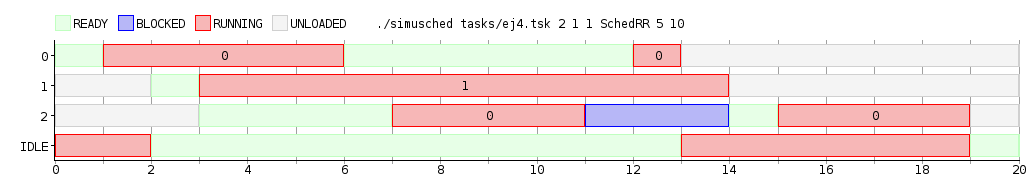
\includegraphics[width=1\columnwidth]{imagenes/ej4.png}
		\caption{\texttt{SchedRR} corriendo 3 tareas con dos núcleos: uno de 5 y
		otro de 10.}
	\end{center}
\end{figure}
